\documentclass[a4paper, 11pt]{article}

% ------------------------------------------------------------------
% Imports
% ------------------------------------------------------------------

% Formatting
\usepackage[landscape, left=.2cm, top=.2cm, right=.2cm, bottom=.2cm]{geometry}
\usepackage{flowfram}
\usepackage[compact]{titlesec}
\usepackage{parskip}
\usepackage{mathptmx} % times font
\usepackage{mathtools}

% Language stuff
\usepackage[english]{babel}
\usepackage[utf8]{inputenc}

% Math imports
\usepackage{amsthm}
\usepackage{amssymb}
\usepackage{amsmath}
\usepackage{bm}
\usepackage{physics}

% Tables
\usepackage{tabularx} % tabularx since the width should be handled automatically

% Graphics
\usepackage{graphics}

% Miscellaneous
\usepackage{hyperref}
\usepackage{enumerate}
\usepackage[inline]{enumitem}
\usepackage{multicol}
\usepackage{xcolor}
\usepackage{etoolbox}
\usepackage{tikz}
\usetikzlibrary{positioning, shapes.multipart, fit}

% ------------------------------------------------------------------
% Formatting
% ------------------------------------------------------------------

% Colors
\definecolor{accent}{HTML}{2563eb}
\definecolor{H1}{HTML}{2ecc71}
\definecolor{H2}{HTML}{3498db}
\definecolor{H3}{HTML}{9b59b6}
\definecolor{H4}{HTML}{e74c3c}
\definecolor{H5}{HTML}{95a5a6}

% Column format
\setlength{\columnsep}{3pt}
\ffvadjustfalse
\Ncolumn{4}
\setlength{\parindent}{0pt}
\setlength{\parskip}{0cm}

% Compact titles
\newcommand{\colorsection}[2]{\colorbox{#1}{\parbox{\dimexpr\linewidth-2\fboxsep}{\centering\ #2}}}
\titlespacing{\section}{0pt}{0pt}{0pt}
\titleformat{\section}{\bfseries\color{white}}{}{0pt}{\colorsection{accent}}

\titlespacing{\subsection}{0pt}{0pt}{0pt}
\titleformat{\subsection}{\bfseries\color{white}}{}{0pt}{\colorsection{black!60}}

% Compact math mode
\makeatletter
\g@addto@macro\normalsize{%
  \setlength{\abovedisplayskip}{0pt}
  \setlength{\belowdisplayskip}{0pt}
  \setlength{\abovedisplayshortskip}{0pt}
  \setlength{\belowdisplayshortskip}{0pt}
  \setlength{\jot}{0pt}
}
\let\displaystyle\textstyle
\makeatother

% Set each display in math mode to be rendered as \textstyle
\renewcommand{\[}{\phantom{}\begin{center}\(}
\renewcommand{\]}{\)\end{center}}

% frames
\usepackage{tcolorbox}
\newenvironment{colored}
{\begin{tcolorbox}[colback=H2!10, colframe=white, boxrule=0.0pt,
                   enlarge top by=-0.1cm, enlarge bottom by=-0.1cm, 
                   enlarge left by=0cm, left=6pt, right=6pt,
                   boxsep=-1.5mm, outer arc=1pt,
                   arc=1pt]}
{\end{tcolorbox}}


% Misc
\hypersetup{colorlinks=true, urlcolor=accent, linkcolor=accent, citecolor=accent}
\setlist{itemsep=0.2pt, topsep=0.5pt, leftmargin=5mm}
\renewcommand{\labelenumii}{\arabic{enumi}.\arabic{enumii}}


% definition environment
\newtheoremstyle{compact_definition}{}{}{\normalfont}{}{\bfseries}{}{0em}{\thmnote{#3}: }
\theoremstyle{compact_definition}
\newtheorem*{definition}{Definition}

% ------------------------------------------------------------------
% Custom Commands
% ------------------------------------------------------------------

% Math general
\newcommand{\R}{\mathbb{R}}
\newcommand{\Q}{\mathbb{Q}}
\newcommand{\N}{\mathbb{N}}
\newcommand{\OB}{\mathcal{O}}
\renewcommand{\iff}{\Leftrightarrow}
\renewcommand{\implies}{\Rightarrow}
% \newcommand{\Z}{\mathbb{Z}}
\newcommand{\C}{\mathbb{C}}
\newcommand{\Pow}{\mathcal{P}}
\newcommand{\argmin}[1]{\text{argmin}_{#1}}
\newcommand{\argmax}[1]{\text{argmax}_{#1}}

% Probability Stuff
\renewcommand{\O}{\Omega}
\renewcommand{\P}{\mathbb{P}}
\newcommand{\PM}{\vb{P}}
\newcommand{\E}{\mathbb{E}}
\newcommand{\F}{\mathcal{F}}
\newcommand{\B}{\mathcal{B}}
\newcommand{\D}{\mathcal{D}}
\newcommand{\I}{1}
\renewcommand{\L}{\mathcal{L}}
\newcommand{\GP}{GP}
\DeclareMathOperator{\KL}{KL}
\DeclareMathOperator{\Var}{\mathbb{V}}
\DeclareMathOperator{\Cov}{Cov}
\DeclareMathOperator{\Ent}{H}
\DeclareMathOperator{\Ber}{Ber}
\DeclareMathOperator{\Bin}{Bin}
\DeclareMathOperator{\NB}{NB}
\DeclareMathOperator{\Geom}{Geom}
\DeclareMathOperator{\Cat}{Cat}
\DeclareMathOperator{\Poisson}{Poisson}
\DeclareMathOperator{\Unif}{\mathcal{U}}
\DeclareMathOperator{\Exp}{Exp}
\DeclareMathOperator{\Normal}{\mathcal{N}}
\DeclareMathOperator{\Laplace}{Laplace}
\DeclareMathOperator{\Ga}{Ga}
\DeclareMathOperator{\Atom}{Atom}
\DeclareMathOperator{\DX}{\mathcal{X}}

% Common Vectors and Matrices
\newcommand{\x}{\vb{x}}
\renewcommand{\r}{\vb{r}}
\newcommand{\y}{\vb{y}}
\newcommand{\z}{\vb{z}}
\newcommand{\w}{\vb{w}}
\newcommand{\Y}{\vb{Y}}
\newcommand{\X}{\vb{X}}
\newcommand{\Z}{\vb{Z}}
\newcommand{\f}{\vb{f}}
\newcommand{\K}{\vb{K}}
\renewcommand{\H}{\vb{H}}
\renewcommand{\k}{\vb{k}}
\renewcommand{\S}{\vb*{\Sigma}}
\renewcommand{\TH}{\vb*{\theta}}
\newcommand{\m}{\vb*{\mu}}
\newcommand{\eps}{\vb*{\epsilon}}
\renewcommand{\I}{\vb{I}}
\newcommand{\0}{\vb{0}}

% Statistical stuff
\DeclareMathOperator{\MSE}{MSE}
\DeclareMathOperator{\MLE}{MLE}
\DeclareMathOperator{\ML}{ML}
\DeclareMathOperator{\MI}{I}

% Misc
\newcommand{\sdots}{\ifmmode\mathinner{\ldotp\kern-0.2em\ldotp\kern-0.2em\ldotp}\else.\kern-0.13em.\kern-0.13em.\fi}
\newcommand{\todo}[1]{{\color{red}\textbf{TODO}: #1}}


% ------------------------
% Document
% ------------------------

\begin{document}

% Title
% \begin{center}
%   \large Probabilistic Artificial Intelligence \\
%   \small \(\langle\)\href{https://google.com}{nicstuder@student.ethz.ch}\(\rangle\)
% \end{center}

% Chapters
\section{Probability Stuff}

% \begin{colored}
%     \textbf{Expectation Dump}

%     \begin{itemize}
%         \item \(\E[\vb{A}\X + \vb{B}\Y + \vb{b}] = \E[\vb{A}\X] + \E[\vb{B}\Y] + \vb{b}\)
%         \item \(\E[\X\Y^\top] = \E[\X] \E[\Y]^\top\) if \(\X \bot \Y\)
%         \item \textbf{LOTUS} \(\E[f(\X)] = \int_{\X(\Omega)} f(\x)p(\x)\,d\x\)
%         \item \textbf{TOWER} \(\E_{\Y} [\E_{\X}[\X \mid \Y]] = \E[\X]\)
%     \end{itemize}
% \end{colored}

\begin{colored}
    % \textbf{Expectation}
        % \(\E[\vb{A}\X + \vb{B}\Y + \vb{b}] = \E[\vb{A}\X] + \E[\vb{B}\Y] + \vb{b}\)
    \(\E[\X\Y^\top] = \E[\X] \E[\Y]^\top\) if \(\X \bot \Y\)
    \(\E[f(\X)] = \int f(\x)p(\x)\,d\x\)
    \textbf{TOWER} \(\E_{\Y} [\E_{\X}[\X \mid \Y]] = \E[\X]\)
\end{colored}

\begin{colored}
    \textbf{Ind.}
    \(\X\bot\Y \iff p(\x\y) = p(\x)p(\y) \iff p(\x \mid y) = p(\x) \)
    % \begin{align*}
    \(\X\bot\Y\mid\Z \iff p(\x, \y \mid \z) = p(\x\mid\z) p(\y \mid \z)
    \iff p(\x \mid \y, \z) = p(\x \mid \z)\)
    % \X\bot\Y\mid\Z &\iff p(\x, \y \mid \z) = p(\x\mid\z) p(\y \mid \z) \\
    % &\iff p(\x \mid \y, \z) = p(\x \mid \z)
    % \end{align*}

    % Reichenbach: \(\forall\X, \Y \exists \Z: \X \not\bot \Y \implies \X \bot \Y \mid \Z\)
\end{colored}

\begin{colored}
    \(\Cov[\X, \Y] = \E[(\X - \E[\X])(\Y - \E[\Y])^\top]\);
    \(\Var[\X + \Y] = \Var[\X] + \Var[\Y] + 2 \Cov[\X, \Y]\);
    \textbf{LOTV} \(\Var[\X] = \E_{\Y}[\Var_{\X}[\X \mid \Y]] + \Var_{\Y}[\E_{\X}[\X \mid \Y]]\);
    \(\Var[\vb{A}\X + \vb{b}] = \vb{A}\Var[\X]\vb{A}^\top\)
\end{colored}

\begin{colored}
    \begin{itemize*}
        % \item \(p(x_{1:i-1}, x_{i+1,n}) = \int_{X_i(\Omega)}p(x_{1:i-1}, x_i, x_{i+1:n}) \,dx_i\)
        \item \textbf{Chain} \(p(x_{1:n}) = p(x_1)\cdot \prod_{i=2}^n p(x_i \mid x_{1:i-1})\) \\
        \item \textbf{LOTP} \(p(\x) = \int_{\Y(\Omega)} p(\x \mid \y) \cdot p(\y) \, d\y\) \\
        \item \(\Y = f(\X) : p(\y) = p_{\X}(f^{-1}(\y)) \cdot |\det Df^{-1}(\y)|\)
    \end{itemize*}
\end{colored}

\begin{colored}
    \textbf{\color{H3} Gauss.}
    \(p(\x) = \frac{\exp\left(-\frac{1}{2}(\x - \m)^\top \S^{-1}(\x - \m)\right)}{(2 \pi)^{n/2} \sqrt{\vert\S\vert}}\)
    % \begin{align*}
    %     \X_A \mid \X_B &= \x_b \sim \Normal (\m_{A \mid B}, \S_{A \mid B}) \ \text{where} \\
    %     \m_{A \mid B} &= \m_A + \S_{AB}\S_{BB}^{-1}(\x_B - \m_B),\\
    %     \S_{A \mid B} &= \S_{AA} - \S_{AB}\S_{BB}^{-1}\S_{BA}.
    % \end{align*}
        \(\X_A \mid \X_B = \x_b \sim \Normal (\m_{A \mid B}, \S_{A \mid B})\)
        where
        \(\m_{A \mid B} = \m_A + \S_{AB}\S_{BB}^{-1}(\x_B - \m_B)\), 
        \(\S_{A \mid B} = \S_{AA} - \S_{AB}\S_{BB}^{-1}\S_{BA}.\)

    % \begin{itemize*}
    %     \item Mean affine f. of \(\m_B\)
    %     \item \(\Var\) can only shrink and does not depend on the observations \(\x_B\).
    % \end{itemize*}

    Equivalently, if \(\X_A\), \(\X_B\) jointly gaussian, then
        \(\X_A = \vb{A}\X_B + \vb{b} + \vb*{\epsilon}\), where
        \(\vb{A} = \S_{AB}\S_{BB}^{-1}\), \\
        \(\vb{b} = \m_A - \S_{AB}\S_{BB}^{-1}\m_B\) and 
        \(\vb*{\epsilon} = \Normal(0, \S_{A \mid B})\)
\end{colored}

\subsection{Bayesian Learning (conditioned on \(\X\))}
\vspace{-8pt}

\[\overbrace{p(\theta \mid \X, \y)}^{\text{Posterior}} = \frac{\overbrace{p(\theta)}^{\text{Prior}} \overbrace{\prod p(y_i \mid \x_i, \theta)}^{\text{Likelihood} \ (p(\y \mid \X, \theta))}}{\underbrace{p(\y \mid \X) ({\scriptscriptstyle = \int p(\theta) \prod p(y_i \mid \x_i, \theta) \, d\theta})}_{\text{Marginal Likelihood ({\color{H4} mostly intracable})}}}\]

\begin{enumerate*}
    \item Define Prior and LL (BLR, GPR)
    \item Predict: \\ \(p(y^\star \mid \x^\star, \X, \y) = \int p(y^\star \mid \x^\star, \theta) p(\theta \mid \X, \y) \, d\theta\)
\end{enumerate*}
\begin{center}
\color{H1}For BLR and GPR, this has a closed form!
\end{center}


\section{Bayesian Linear Regression}

\textbf{Idea}: Reason \(\w\)'s \textit{full posterior}, not only mode.

\begin{definition}[Model]
    \(y_i = {\w^\star}^\top \x_i + \epsilon_i\) with \(\epsilon_i \sim \Normal(0, \sigma_n^2)\) or equivalently \(y_i \mid \x_i, \w \sim \Normal(\w^\top \x_i, \sigma_n^2)\).
    With this model we find \(\hat\w_{\text{MLE}}  = \hat\w_{\text{ls}}\).
\end{definition}

\begin{colored}
    \textbf{Ridge Interpretation}: Ass. \(\w \sim \Normal(\0, \sigma_p^2\I)\), \(\w \bot \x_{1:n}\), \(y_i \bot y_j \mid \x_{1:n}, \w\). Then log-posterior is
    \(\log p(\w \mid \x_{1:n}, y_{1:n}) = -\frac{1}{2} [\w^\top \S \w - 2\m] + \text{const}\) \\
    w/ \(\S = (\sigma_n^{-2}\X^\top\X + \sigma_p^{-2}\I)^{-1}\), \(\m=\sigma_n^{-2}\S\X^\top\y\).
    Note we used \(p(\w \mid \y, \X) = \frac{p(\y \mid \X, \w)p(\w)}{p(\y\mid\X)}\), where we condition everywhere on \(\X\), but \(\w \bot \X\).
    \textbf{MAP}: \(\hat\w_{\text{MAP}} = \text{argmin}_{\w} \norm{\y - \X\w}_2^2 + \frac{\sigma_n^2}{\sigma_p^2}\norm{\w}_2^2\).
    \(\hat\w_{\text{ridge}} = (\X^\top\X + \lambda \I)^2 + \lambda\norm{\w}_2^2 \quad (\X\in\R^{n \times d})\)
    Note if \(\w \sim \Laplace(\0, l) \implies \lambda = \sigma_n^2/l\).
\end{colored}

MAP approximates full posterior by placing all mass on its mode, BLR predicts by averaging.

\begin{definition}[Inf.]
    \resizebox{0.88\linewidth}{!}{\(y^\star \mid \x^\star, \x_{1:n}, y_{1:n} \sim \Normal(\mu^\top \x^\star, {x^\star}^\top \S \x^\star + \sigma_n^2)\)}

    \resizebox{\linewidth}{!}{\(\Var[y^\star \mid \x^\star] = \underbrace{\E_\theta[\Var_{y^\star}[y^\star \mid \x^\star, \theta]]}_{\text{Aleatoric (Data)}} + \underbrace{\Var[\E_{y^\star}[y^\star \mid \x^\star, \theta]]}_{\text{Epistemic (Model)}}\)}
\end{definition}

\subsection{Kernelized BLR}
\begin{definition}[Kernelized BLR] (\(\Phi = \phi(\X)\), prior \(\w \sim \Normal\))
    \(\f \mid \X \sim \Normal(\Phi \E[\w], \Phi\Var[\w]\Phi^\top) = \Normal(\0, \K)\), with \(\K = \sigma_p\Phi\Phi^\top\), hence \(k(\x, \x') = \Cov[f(\x), f(\x')]\).
\end{definition}

Conditions for a valid kernel function \(k\): \\
\begin{itemize*}
  \item \(k(x, z) = k(z, x)\)
  \item \(K\) psd s.t. \(\forall x. \ x^\top K x \geq 0 \)
\end{itemize*}

\begin{definition}[Inner Product kernel]
  \(k(x, z) = h(\langle x, z \rangle)\)
\end{definition}

\begin{definition}[Poly ker.]
  \(k(x, z) = (c_{\geq 0} + \langle x, z \rangle)^m\), \(d_\phi = \binom{d + m}{d}\)
\end{definition}

\begin{definition}[RFB kernel]
  \(k(x, z)  = \exp\left(\frac{||x - z||_2^\alpha}{\tau}\right)\) which is \textbf{Gaussian} \(: \alpha = 2\), \textbf{Laplacian} \(: \alpha = 1\). \(d_\phi = \infty\)
\end{definition}

\begin{definition}[Kernel Composition]
  \begin{itemize*}
    \item \(k_1 \dotplus k_2\)
    \item \(c\cdot k \ (c >0)\)
    \item \(k((x \ y), (x' \ y')) = k_1(x \ x') \dotplus k_2(y \ y') \)
    \item \(f(k)\) for any poly. \(f\) with positive coeff or \(f = \exp\)
  \end{itemize*}
\end{definition}

\begin{definition}[Stationary]
  \(\iff \exists \tilde k: \tilde k (\x - \x') = k(\x, \x')\)
\end{definition}

\begin{definition}[Isotropic]
  \(\iff \exists \tilde k: \tilde k (\norm{\x - \x'}_2) = k(\x, \x')\)
\end{definition}


\section{Gaussian Processes}

\begin{definition}[GP]
    Infinite RVs \(\DX\), any finite num. of which are jointly Gaussian. Prior \(f \sim \GP(\mu, k)\).

    % Given \(\mu\) and \(k\) and using homoscedastic noise:
    % \[y^\star \mid \x^\star, \mu, k \sim \Normal(\mu(\x^\star), k(\x^\star, \x^\star) + \sigma_n^2)\]
\end{definition}

% \begin{definition}[Inference]
%     Given prior \(f \sim \GP(\mu, k)\), noisy obs. \(\y\) (\(y_i = f(\x_i) + \epsilon_i\)) and noise-free pred. \(f^\star\) at \(\x^\star\), joint Gauss.: \(\begin{bmatrix}
%         \y \\ f^\star 
%     \end{bmatrix}\mid \x^\star, \x_{1:n} \sim \Normal(\tilde\m, \tilde\K)\)

%     \resizebox{\linewidth}{!}{\(
%         \tilde\m = \begin{bmatrix}
%             \m_A \\
%             \mu(\x^\star)
%         \end{bmatrix}, \qquad
%         \tilde\K = \begin{bmatrix}
%             \K_{AA} & \k_{\x^\star, A} \\
%             \k_{\x^\star, A}^\top & k(\x^\star, \x^\star)
%         \end{bmatrix}, \qquad
%         \k_{\x^\star, A} = \begin{bmatrix}
%             k(\x^\star, \x_1) \\
%             \vdots \\
%             k(\x^\star, \x_n)
%         \end{bmatrix}
%     \)}
% \end{definition}

\begin{definition}[Inference]
    Obs. \(y_i = f(\x_i) + \epsilon_i\), \(\epsilon_i \sim \Normal(0, \sigma_n^2)\)
    Use {\color{H3} cond. multiv. Gauss.} for closed form post.:
    \(f^\star \mid \X, \y \sim \GP(\mu', k')\) with updated:
    \begin{align*}
        \mu'(\x) &= \mu(x) + \k_{\x, A}^\top(\K_{AA} + \sigma_n^2\I)^{-1}(\y_A - \mu_A) \\
        k'(\x, \x') &= k(\x, \x') - \k_{\x, A}^\top (\K_{AA} + \sigma_n^2\I)^{-1}\k_{\x', A}.
    \end{align*}
\end{definition}

\begin{definition}[Forward Sampling]
    Sample recursively: \\
    \(p(\x_1, \ldots, \x_n) = p(f_1)p(f_2 \mid f_1)\ldots p(f_n \mid f_{1:n})\)
\end{definition}

\subsection{Optimizing Kernel Params}

\begin{definition}[Max. Marginal Likelihood]
    Optimize effects of params \(\theta\) over all \(f\). For GP-Regression:
    \[y_{1:n} \mid \x_{1:n}, \theta \sim \Normal(\0, \K_{f, \theta} + \sigma_n^2\I),\]
    with \(\K_{f, \theta}\) matrix at \(\x_{1:n}\) by using \(\theta\). Then
    \begin{align*}
        \hat\theta_{\text{MLE}} &= \argmax{\theta} p(y_{1:n} \mid \x_{1:n}, \theta) \\
        &=\argmax{\theta} \Normal(\y; \0, \K_{\y, \theta} ({\scriptstyle = \K_{f, \theta} + \sigma_n^2\I})) \\
        &= \argmin{\theta} \underbrace{\frac{1}{2}\y^\top \K_{\y, \theta}^{-1} \y}_{\text{Fit}} + \underbrace{\frac{1}{2} \log\det(\K_{\y, \theta})}_{\text{Volume}}
    \end{align*}
    Using full posterior would be intractable.
\end{definition}

\begin{definition}[Empirical Bayes]
    with \(\vb{\alpha} = \K_{\y, \theta}^{-1}\y\):

    \resizebox{\linewidth}{!}{
        \(\partial_{\theta_j}\log p(y_{1:n} \mid \x_{1:n}, \theta) = \frac{1}{2} \tr\left((\vb{\alpha}\vb{\alpha}^\top - \K_{\y, \theta}^{-1})\partial_{\theta_j}\K_{\y, \theta}\right)\)
    }
\end{definition}

\subsection{Approximations as GP \(\in \OB(n^3)\)}

\begin{definition}[Local methods]
    Condition on: \(|k(x, x')| \geq \tau\). Still expensive if many points close by.
\end{definition}

\begin{definition}[Kernel Function Approximation]
    Approx. \(k\) with low-dim. map  \(k(\x,\x') \approx \phi(\x)^\top\phi(\x')\) using e.g. RFF.
    Then apply BLR in \(\OB(nm^2 + m^3)\).
\end{definition}

\begin{definition}[RFF]
    Stationary \(k\) can be interpreted with FT: \(k(\x-\x') = \int_{\R^d} p(\omega) e^{i \omega^\top(\x - \x')} \, d\omega\)
\end{definition}

\begin{definition}[Inducing Points]
    Get \(f\) vals at points by sampling/heuristic/equal space/hyperp. SoR, FITC.
\end{definition}

\section{Variational Inference}

\begin{definition}[Idea]
    Approximate intractable posterior \[p(\theta \mid \X, \y)\]
\end{definition}

\section{Markov Chain Monte Carlo}

\begin{definition}[Idea]
    Use \(p(y^\star \mid \x^\star, \X, \y) \overset{\text{LLN}}{\approx} \underbrace{\frac{1}{m}\sum p(y^\star \mid \x^\star, \theta^{(i)})}_{\approx \E_{\theta \mid \X, \y}[p(y^\star \mid \x^*, \theta)]}\)

   \vspace{-15pt} and MC to sample posterior.
\end{definition}

\begin{definition}[MC]
    Over states \(S = [n]\) is sequence of RVs s.t.
    \begin{itemize*}
        \item \(P(X_{t+1} \mid X_t)\) independent of \(t\)
        \item \(X_{t+1} \bot X_{1:t-1} \mid X_t\)
    \end{itemize*}
\end{definition}

\begin{definition}[Stationary]
    \(\pi(x) = \sum_{x'} p(x \mid x')\pi(x')\)
\end{definition}

\begin{definition}[Irreducible]
    \(\forall s, s' \in S: \P[s \to s'] > 0\)
\end{definition}

\begin{definition}[Ergodic]
    \(\exists t \in \N_0\) s.t. every state can be reached from every state in exactly \(t\) steps.
\end{definition}

Irreducible \(\to\) Ergodic: \(\PM' = \frac{1}{2}\PM + \frac{1}{2}\I\)

\begin{colored}
    Ergodic MC has unique stat. \(\pi\) (with full support) and \(\lim_{t \to \infty q_t} = \pi\), independently of \(q_0\).
\end{colored}

\begin{definition}[Detailed Balance]
    If MC satisfies \(\frac{1}{Z}q(x)p(x'\mid x) = \frac{1}{Z}q(x')p(x \mid x')\), then \(\frac{1}{Z}q(x)\) is stat. dist.
\end{definition}

% \begin{definition}[Ergodic Theorem]
%     For an ergodic MC and stat. dist \(\pi\), as well as \(f: S \to \R\), then \(\frac{1}{n} \sum f(x_i) \overset{\text{a.s.}}{\to} \sum_{x \in S} \pi(x)f(x) = \E_{x \in \pi}[f(x)]\) for \(x_i \sim X_i \mid x_{i-1}\).
% \end{definition}
\vspace{-12pt}
\[\color{H2}p(y^\star \mid \x^\star, \X, \y) \approx \frac{1}{T - t_0}\sum_{i = t_0 +1}^T p(y^\star \mid \x^\star, \theta^{(i)})\]

\subsection{Transition Distributions}

\begin{colored}
    \textbf{Metro. Hast.} \(\alpha(x'\mid x) = \min\left\{1, \frac{q(x') r(x\mid x')}{q(x) r(x' \mid x)}\right\}\)
    \begin{enumerate*}
        \item Sample \(x' \sim r(x' \mid x)\)
        \item Accept w/ prob. \(\alpha\)
    \end{enumerate*}
    Stationary dist. is \(\frac{1}{z}q(x) = p(x)\).
\end{colored}

\begin{definition}[Gibbs S.]
    Pick \(i \in [n]\), update \(x_i\) by sampling according to \(r(x' \mid x) = p(x_i \mid \x_{-i})\).
    \(\alpha(x' \mid x) = 1\)
\end{definition}

\begin{definition}[Continuous Case]
    Focus on \textit{Gibbs Distributions} of the form \(p(\x) = \frac{1}{Z}\exp(-f(\x))\) w/ energy function \(f\). If \(f\) convex \(p\) is log-concave.
    \(\alpha(x'\mid x) = \min \left\{1, \frac{r(x \mid x')}{r(x' \mid x)} \exp(f(x) - f(x'))\right\}\)
\end{definition}

\begin{definition}[Langevin Dynamics]
    Shift proposal distribution perpendicular to the gradient of the energy:
    \(r(x' \mid x) = \Normal(x'; x - \eta_t \nabla f(x), 2\eta_t \I)\).
\end{definition}


\section{Bayesian Deep Learning}

\begin{definition}[BNN]
    \resizebox{.85\linewidth}{!}{\(\theta \sim \Normal(\0, \sigma_p^2\I)\),\(y \mid \X, \theta \sim \Normal({\color{H2}f(\x, \theta)}, \sigma_n^2)\)}
    GA: \(\theta \leftarrow \theta(1 - \frac{1}{\sigma_p^2}\eta_t) + \eta_t \sum\nabla\log p(y_i \mid \x_i, \theta)\)
\end{definition}

\begin{definition}[Heteroscedastic Noise] Use complex likeli-\\hood:
    \(y \mid \X, \theta \sim \Normal({\color{H2}f_\mu(\x, \theta)}, \exp({\color{H3}f_{\sigma^2}(\x, \theta)}))\)
    \textbf{MAP}:
    \(\arg\min_\theta \lambda \Vert \theta \Vert_2^2 - \frac{1}{2}\left[\log {\color{H3}f_{\sigma^2}}+ \frac{(y_i - {\color{H2}f_\mu})^2}{\color{H3}f_{\sigma^2}}\right]\)

    \begin{enumerate*}
        \item prior
        \item penalize big \(\sigma\)
        \item penalize error on \(\mu\)
    \end{enumerate*}
\end{definition}

\subsection{Approximate Inference (heteroscedastic)}

% Want epistemic uncertainty -- but {\color{H4}intractable} if no homoscedastic noise.

\begin{definition}[Bayes by Backprop]
VI for BNNs.
Pred post dist \(q\) instead of value (VI).
Optimize ELBO via SGD / For Gaussian \(q(\theta \mid \lambda) = \Normal(\theta; \mu, \Sigma)\),

\resizebox*{\linewidth}{!}{
    \(\nabla_\lambda L(\lambda) = \nabla_\lambda \E_{\theta \sim q(\cdot \mid \lambda)}[\log p(y \mid \theta)] - \nabla \lambda \KL(q_\lambda \Vert p(\cdot))\)
}

\(\approx \nabla_{C, \mu}\E_{\epsilon \sim \Normal(0, \I)}[\log p(y \mid C\epsilon + \mu)]\) \\ \(+ \nabla_{C, \mu}\KL(q_{C, \mu} \mid p(\cdot))\)
w/ \(\theta^{(j)} = C\epsilon^(j) + \mu, x_{i_j}\).
\end{definition}

\begin{definition}[MCMC]
    SGLD / SG-HMC on \(\color{H2}p(y^\star \mid \x^\star, \X, \y)\). Store \(m < T\) (\textit{subsampling}) or approx. weights by learning \(\theta \sim \Normal(\m, \S)\), where
    \(\m = \frac{1}{T}\sum \theta^{(i)}\), \(\S = \frac{1}{T-1}\sum (\theta^{(i) - \m})(\theta^{(i)} - \m)^\top\) (SGD \(\scriptstyle\to\){\color{H1}SWAG}).
\end{definition}

\begin{definition}[Dropout]
    VI with \(q(\theta\mid\lambda) = \prod q_j(\theta_j \mid \lambda_j)\) w/ \(q_j(\theta_j \mid \lambda_j) = p \delta_0(\theta_j) + (1 - p)\delta_{\lambda_j}(\theta_j)\)
\end{definition}

\begin{definition}[Probabilistic Ensembles]
    Train multiple models on random subsamples of data.
\end{definition}

\begin{definition}[Calib. Err.]
    \(\text{ECE} = \sum_{m=1}^M \frac{\vert B_m}{m} \vert \text{fr}(B_m) - \text{cf} (B_m) \vert\), \(\text{fr}(B_m) = \frac{1}{\vert B_m \vert} \sum_{i} \vb{1}(\hat y_i = 1)\), \(\text{cf}(B_m) = \frac{1}{\vert B_m \vert} \sum_{i} \hat p_i\)
\end{definition}


\section{Active Learning}

Query points that provide useful information.

\begin{colored}
    \(\Ent[\X, \Y] = \E_{(\x,\y)}[-\log p(\x, \y)]\),
    \(\Ent[\X\mid\Y] = \E_{\y}[\Ent[\X \mid \Y = \y]] = \E_{(\x,\y)}[-\log p(\x \mid \y)]\)
    \begin{itemize}
        \item \(\Ent[\X, \Y] = \Ent[\Y] + \Ent[\X \mid \Y]\)
        \item \(\Ent[\X \mid \Y] = \Ent[\Y \mid \X] + \H[\X] - \H[\Y]\) (Bayes)
        \item \(\Ent[\X\mid\Y] \leq \Ent[\X]\) (Information never hurts)
    \end{itemize}
\end{colored}

\begin{colored}
    \textbf{Mutual Info}
    \(\MI(\X; \Y) = \Ent[\X] - \Ent[\X \mid \Y]\)
    Loss of entropy after obs. \(\MI(\X;\Y) \geq 0\) (Info never hurts)
    \(\MI(\X; \Y \mid \Z) = \Ent[\X \mid \Z] - \Ent[\X \mid \Y, \Z]\)
\end{colored}

% \begin{definition}[Mar. Gain]
%     \(\x \in \DX\), \( A\subseteq \DX\), \(F: \mathcal{P}(\DX) \to \R\):
%     \begin{gather*}
%     \Delta_F(\x \mid A) = F(A \cup \{\x\}) - F(A) \\
%     \end{gather*}
% \end{definition}

% \vspace{-15pt}
% \begin{definition}[Submodular]
%     \(\iff \forall \x \in \DX, A \subseteq B \subseteq \DX:\)
%     \begin{gather*}
%         F(A \cup \{\x\}) - F(A) \geq F(B \cup \{\x\}) - F(B)
%     \end{gather*}
%     \textit{Monotone} if \(F(A) \leq F(B)\)
% \end{definition}

\begin{definition}[Maximization Objective (Info. Gain)]\ \\
    \(\MI(S) = I(\f_S; \y_S) = \overbrace{\Ent[\f_S]}^{\mathclap{\hspace{-60pt}\text{Uncertainty before eval}}} - \overbrace{\Ent[\f_S \mid \y_S]}^{\mathclap{\text{After evaluating } \y_S}} \to\)
    NP-hard.
\end{definition}

\begin{definition}[Greedy Algorithm]
    Pick \(\x \in S\), which maximizes mutual information \(I(S \cup \{\x\})\)
\end{definition}

\begin{definition}[Uncertainty Sampling]
    If \(f\) is Gauss \& hetero: \(\x_{t+1} \in \argmax{x} \frac{\sigma_p^2(x)}{\sigma_n^2(x)}\). Homo: \(\argmax{x} \sigma_p^2(x)\).
\end{definition}

\begin{definition}[Classification]
    \textit{US} is max. \(\Ent\) of predicted label:
    \(\x_{t+1}\in\argmax{\x}\Ent(y_{\x} \mid \X,\y)\)
\end{definition}

\begin{definition}[BALD]
    Select points where models are confident, but different:
    \(\x_{t+1} = \argmax{\x} \MI(\theta;y_{\x} \mid \X, \y) = \argmax{\x} \Ent[y_{\x} \mid \X, \y] - \E_{\theta \mid \X, \y}[\Ent[y_{\x} \mid \theta]]\)
\end{definition}
\section{Bayesian Optimization}
Not only learn, but also optmimize for reward.

\begin{definition}[Regret]
    \(R_T = \sum(\max_{\x} f^\star(\x) - f^\star(\x_t))\)
    Goal is to get sublinear regret \(\frac{R_T}{T} \to 0\) \(\to\) gain info
\end{definition}

\begin{definition}[BO-GP]
    \begin{enumerate*}
        \item init \(f \sim \GP\)
        \item choose new point \(\x_t = \argmax{}F(\x; \mu_{t-1}, k_{t-1})\)
        \item \(\y_t = f(\x_t) + \epsilon_t\)
        \item Update \(\mu_t, k_t\)
    \end{enumerate*}
    ({\color{H5} \(F\) acqui. func. (e.g. US, UCB)})
\end{definition}

\begin{definition}[UCB]
    \(\x_{t+1} = \argmax{} \mu_t(\x) + \beta_{t+1} \sigma_t(\x)\) with \\ \(\color{H3}\sigma_t(\x) = \sqrt{k_t(\x,\x)}\), \(\beta=0\): exploit., \(\beta \to \infty\): US.
    {\color{H4} Non-convex: Lipschitz optim. or GA}
\end{definition}

\begin{colored}
    \textbf{GP-UCB Regret}: \(\frac{1}{T}R_T = \OB^*(\sqrt{\frac{\gamma_T}{T}})\) where
    \(\gamma_T = \max_{|S| \leq T} \MI(f_S; \y_S)\) is information gain.
    Info. gain bounds for common kernels:
    \begin{itemize}
        \item \textit{Linear}: \(\gamma_T = \OB(d \log T)\)
        \item \textit{Gaussian}: \(\gamma_T = \OB((\log T)^{d+1})\)
        \item \textit{Matérn}: \(\gamma_T = \OB(T^{\frac{d}{2\nu + d}} (\log T)^{\frac{2\nu}{2\nu + d}})\)
    \end{itemize}
\end{colored}

\begin{definition}[PI]
    % \(\x_{t+1} = \argmax{} \P(I_t(\x) > 0 \mid \X, \y) = \argmax{} \Phi(\frac{\mu_t(\x) - \hat f_t}{\sigma_t(\x)})\)
    \(\x_{t+1} = \argmax{} \Phi(\frac{\mu_t(\x) - \hat f_t}{\sigma_t(\x)})\)
\end{definition}

\begin{definition}[EI]
    \(\x_{t+1} = \argmax{} \E[I_t(\x) \mid \X, \y] \, ({\scriptstyle I_t = (f(\x) - \hat f_t)_+})\)
    Has weird non-linearities.
\end{definition}

\begin{definition}[Thompson Sampling]
    At time \(t+1\), sample \(\tilde f_{t+1} \sim p(\cdot \mid \X, \y)\) from post. The, simply max \(\tilde f_{t+1}, \x_{t+1} = \argmax{} \tilde f_{t+1}(\x)\).
\end{definition}


\section{Markov Decision Processes}

\begin{definition}[MDP]
    States \(X\), Actions \(A\), \textit{\color{H2} known} Trans. Prob. \(p(x' \mid x, a)\) and reward f. \(r: X \times A \to \R\).
\end{definition}
\begin{center}
    Stochastic env. \(\iff\) output of \(a\) is random.
\end{center}

\begin{definition}[Policy]
    \(\pi(a \mid x)\) prob. dist. over actions. Induces MC:
    \(p^\pi(x'\mid x) = \sum_a \pi(a \mid x) p(x' \mid x, a)\).
\end{definition}

\begin{definition}[Discounted Payoff]
    \(G_t = \sum_{m=0}^\infty \gamma^m R_{t + m}\)
\end{definition}

\begin{definition}[St. V. F.]
    \(v_t^\pi(x) = \E_\pi[G_t \mid X_t = x] = q^\pi(x, \pi(x))\)
\end{definition}

\begin{definition}[St. V-A./Q]
    \(q_t^\pi(x, a) = \E_\pi[G_t \mid X_t = x, A_t = a]\) \\ \(= r(x, a) + \gamma \sum_{x'}p(x' \mid x, a) v_{t+1}^\pi(x')\)
\end{definition}

\begin{definition}[Stochastic Bellmann Equations] \, \\
    \begin{enumerate*}
        \item \resizebox{.95\linewidth}{!}{
            \(v^\pi(x) = r(x, \pi(x)) + \gamma\sum_{x'}p(x' \mid x, \pi(x)) v^\pi(x')\)
        }
        \item \resizebox{.95\linewidth}{!}{
            \(v^\pi(x) = \sum_a \pi(a \mid x)\left(r(x, a) + \gamma\sum_{x'}p(x' \mid x, a) v^\pi(x')\right)\)
        }
        \item \resizebox{.95\linewidth}{!}{
            \(q^\pi(x, a) = r(x, a) + \gamma \sum_{x'}p(x' \mid x, a) \sum_{a'} \pi(a' \mid x') q^\pi(x', a')\)
        }
        \item \(v^\star(x) = \max_a[r(x, a) + \gamma \sum_x' p(x' \mid x, a) v^\star(x')]\)
        \item \(q^\star(x, a) = r(x, a) + \gamma \sum_{x'} p(x' \mid x, a) v^\star(x')\)
    \end{enumerate*}

    { \color{H1} Allows us to define state-values from the next!} \(\implies\) find \(v^\pi\), given policy \(\pi\).
\end{definition}

\begin{definition}[Pol.-Eval.]
    BE \(\implies v^\pi = (\I - \gamma \vb{P}^\pi)^{-1}\r^\pi\), solve iter. with \(v^\pi \leftarrow \r^\pi + \gamma \PM^\pi v^\pi\)
\end{definition}

\begin{definition}[Pol.-Opt.]
    Find \(\pi^\star = \argmax{}\E_{\pi}[G_0]\), which is greedy w.r.t. s.v.f.: \(\pi^\star(x) = \argmax{a} q^\star(x, a)\).
\end{definition}

\begin{definition}[PI]
    rand \(\pi_0 \overset{\text{PE}}{\to} v_0 \overset{\text{PO}}{\to} \pi_1 \overset{\text{PE}}{\to} \ldots \pi^\star\). Take poly-\# steps, converge to optimal policy, \(\OB(n^3)\).
\end{definition}

\begin{definition}[VI]
    BE4 with DP, start with \(v_0(x) = \max_a r(x, a)\).
    \(\epsilon\)-opt sol in poly-\# steps, \(\OB(nm)\). Non-\(\nearrow\).
\end{definition}

\begin{definition}[POMDP]
    \(p(y \mid b_t, a_t) = \sum_{x, x'}b_t(x) p(x' \mid x, a_t)p(y \mid x')\);
    \(b_{t+1}(x') = \frac{1}{Z} \sum_x b_t(x)p(x' \mid x, a_t)p(y_{t+1} \mid x')\)
    For finite horizon \(T\), set of reachable belief states is finite but exponential in \(T\).
\end{definition}
\section{Tabular Reinforcement Learning}

\begin{definition}[On-Policy]
    % Learn using current policy's data.
    Learn and act using same policy
    % Agent has control over its own actions.
    % Update policy based on data collected using current policy only
\end{definition}

\begin{definition}[Off-Policy]
    % Learn using any policy's data.
    Learn policy using anothers' data.
    % Use purely obervational data.
    % Update policy based on data collected using any policy.
\end{definition}

\subsection{Model-Based (learn \(p(x' \mid x, a)\) of MDP)}

off-policy.  Mem: \(\OB(n^2m)\), Compt: \(\OB(nm)\)

\begin{definition}[MC-Control]
    \(\hat p(x' \mid x, a) = \frac{N(x' \mid x, a)}{N(a \mid x)}\) for MLE and \(\hat r(x, a) = \frac{1}{N(a \mid x)} \sum_{t=0, x_t = x, a_t = a}r^t\)
\end{definition}

\begin{definition}[\(\epsilon\)-greedy]
    \begin{enumerate*}
        \item \(u \sim \Unif\)
        \item \(u \leq \epsilon_t\): rand \(a\), else best
    \end{enumerate*}
\end{definition}

\begin{definition}[\(\bm R_{\max}\)]
    Add state \(x^\ast\) and set \(\forall x, a: \hat r(x, a) = R_{\max}\), \(\hat p(x^* \mid x, a) = 1\), then compute optimal policy \(\hat\pi\).
    Quickly eliminate suboptimal, with prob \(1 - \delta\), reaches \(\eps\)-opt policy, \(\#\) of steps poly. in \(|X|, |A|, T, \frac{1}{\epsilon}, \log(\frac{1}{\delta}), R_{\max}\).
\end{definition}

% TODO: Might add softmax exploration

\subsection{Model-Free (learn \(v\) directly)}

\begin{definition}[Bootstrapping]
    Approx. \(v^\pi(x) \approx r + \gamma v^\pi(x')\) using estimate \(V^\pi\), which itself samples \(v^\pi\).
\end{definition}

\begin{definition}[TD-learning]
    % \begin{enumerate*}
    %     \item \(V^\pi\) arb.
    %     \item use \(\pi\): \((x, a, r, x')\)
    %     \item \(V^\pi(x) = (1 - \alpha_t)V^\pi(x) + \alpha_t(r + \gamma V^\pi(x'))\)
    % \end{enumerate*}
    \textit{on-policy}, \(\alpha^t\) (*) \(V^\pi \to v^\pi\) with prob 1.
    Use bootstrapping to reduce variance
    \(V^\pi(x) = V^\pi(x) + \alpha_t(r + \gamma V^\pi(x') - V^\pi(x))\).
\end{definition}

\begin{definition}[SARSA]
    TD with \(Q^\pi(x, a) = (1 - \alpha_t) Q^\pi(x, a) + \alpha_t(r + \gamma Q^\pi(x', a'))\)
\end{definition}

\begin{definition}[Q-learning]
    \textit{Off-policy}, same conv. cond, bootstrapped. Mem \(\OB(nm)\), Compt. \(\OB(m)\).\\
    \resizebox{\linewidth}{!}{
    \(Q^\star(x, a) = (1 - \alpha_t)Q^\star(x, a) + \alpha_t(r + \gamma \max_{a'}Q^\star(x', a'))\)
    }
\end{definition}

\section{Non-Tabular Model-Free RL}

\begin{definition}[Idea]
    Approx \(V, Q\) without \(\OB(n), \OB(nm)\) space.
\end{definition}

% stochastic gradient descent with a bootstrapping estimate is also called stochastic-semi-gradient descent.
\begin{definition}[TD as SGD]
    \resizebox{0.72\linewidth}{!}{
    \(l_2(\TH; x, r, x') = \frac{1}{2} (r + \gamma \TH^{\text{old}}(x') - \TH(x))^2\)
    }
\end{definition}

% \begin{itemize}[leftmargin=*]
%     \item \(\delta_{\text{TD}} = r + \gamma \TH^{\text{old}}(x') - \TH(x)\)

% \end{itemize}


\begin{definition}[Q-Learn. w/ F.A.]
    \(\TH \leftarrow \TH - \alpha_t \delta_* \nabla_{\TH} Q^\star(x, a;\TH)\)
    Upd. \(\TH^{\text{old}}\) aft. \(|\D|\) stp. \(l_2(\TH) = \frac{1}{2}\sum_{d \in \D}(\delta_*(d))^2\)
    \begin{itemize}[leftmargin=*]
        \item \hspace{-2pt}\resizebox{1.01\linewidth}{!}{
        \(\delta_{\text{DQN}} = { r + \gamma \max_{a'} Q^\star(x', a'; \TH^{\text{old}}) - Q^\star(x, a; \TH)}\)
        } \\ % note that the update of the online-network still happens with a random sample of the replay buffer. the summation is implicit.
        It suffers from maximization bias.
        \item \hspace{-2pt}\resizebox{1.01\linewidth}{!}{
        \(\delta_{\text{DDQN}} = { r + \gamma Q^\star(x', a^\star(x';\TH); \TH^{\text{old}}) - Q^\star(x, a; \TH)}\)
        } \\
        where \(a^\star(x'; \TH) = \argmax{a'}Q^\star(x', a';\TH)\)
    \end{itemize}
\end{definition}

\subsection{Policy Gradient Methods \(\pi^\star(x) \approx \pi_\varphi(x)\)}

\begin{center}
    \(j(\pi) = \E_\pi[G_0], \quad \nabla_\varphi j(\varphi) \approx {\color{H2}\nabla_\varphi \E_{\tau \sim \Pi_\varphi}[G_0]}\) \\
    \(\Pi_\varphi(\tau) = p(x_0) \Pi_{t=0}^{T-1} \pi_\varphi(a_t \mid x_t) p(x_{t+1} \mid x_t, a_t)\)
\end{center}

\begin{definition}[Score-Gr-Est]
    \({\color{H2} \E_{\tau \sim \Pi_\varphi}[(G_0 - b)\nabla_\varphi \log \Pi_\varphi(\tau)]}\)
\end{definition}

\begin{definition}[REINFORCE]
    SGE with downstream return:
    \(\varphi \leftarrow \varphi + \eta {\color{H2}\gamma^t g_{t:T} \nabla_\varphi \log \pi_\varphi(a_t \mid x_t)}\)
\end{definition}

\begin{definition}[Adv. F.]
    \(a^\pi(x, a) = q^\pi(x, a) - v^\pi(x)\)
\end{definition}

\begin{definition}[PG-Thm]
    Use VF-est. with PGM (online)

    % \resizebox{\linewidth}{!}{
    %     \(\nabla_\varphi j(\varphi) = \sum_{0}^\infty \E_{x_t, a_t}[\gamma^t q^{\pi_\varphi}(x_t, a_t) \nabla_\varphi \log \pi_\varphi(a_t \mid x_t)]\)
    % }
    \begin{center}
    \(\nabla_\varphi j(\varphi) = \E_{(x, a) \sim \pi_\varphi}[q^\pi_\varphi(x, a) \nabla \log \pi_\varphi(a \mid x)]\)
    \end{center}
\end{definition}

\subsection{Actor-Critic}
\begin{center}
    \textit{Actor} (\(\pi\)-app. [PG-T]), \textit{Critic} (\(Q\)-app. [TD])
\end{center}

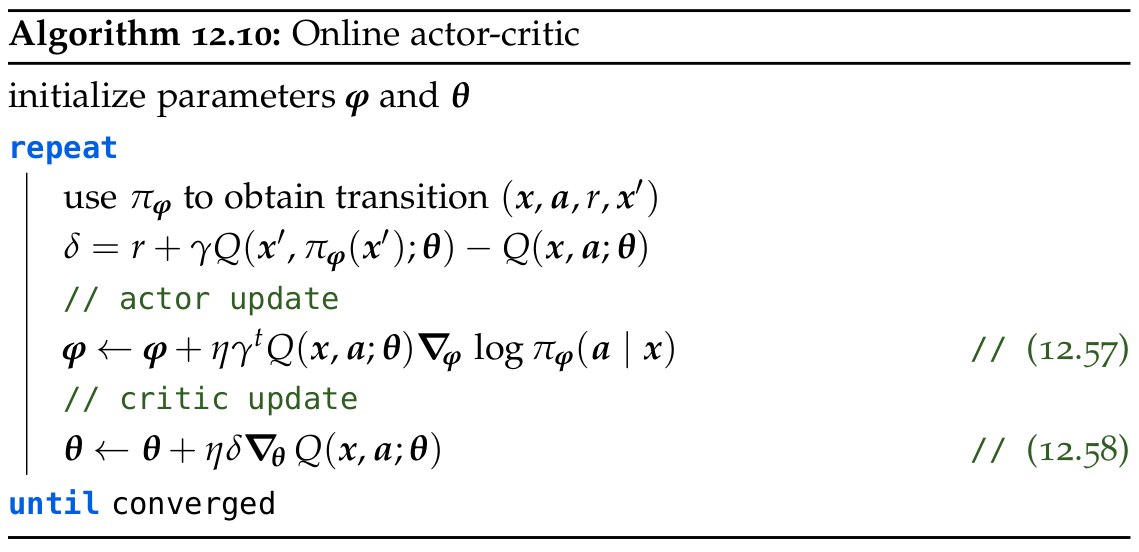
\includegraphics[width=\linewidth]{assets/actor_critic.png}

\begin{definition}[A2C]
    \(Q(x, a; \TH) \to A(x, a; \TH)\) for \(\varphi\)
\end{definition}

\begin{definition}[TRPO]
    Opt. surrogate obj. withing trust region
\end{definition}

\begin{definition}[PPO]
    Effective heuristic variant of TRPO
\end{definition}

\begin{definition}[\color{H2}DDPG]
    Combines DQN with reparam PG
\end{definition}

\begin{definition}[\color{H2}TD3]
    Extension of DDPG to avoid max. bias
\end{definition}

\begin{definition}[\color{H2}SAC]
    Variant of DDPG for \(\Ent\)-regularized MDP
\end{definition}

\begin{definition}[Repa. Policy]
    \(a \sim \pi(x; \TH_\pi) \to a \sim \phi(x; \TH_\pi, \eps)\), deterministic policy + indepenent noise.
\end{definition}

\section{Model-Based RL}
Start wiht init \(\pi\) and data \(\mathcal{D}\). For several eps:
\begin{enumerate}
    \item Roll outpolicy \(\pi\) to collect data
    \item Learn dynamics \(f\) and rewards \(r\) from data
    \item Plan new \(\pi\) based on estimated models
\end{enumerate}

\begin{definition}[MPC]
    \begin{enumerate*}
        \item Observe \(x_t\)
        \item Plan over finite Horizon \(\max_{a_{t:t+H-1}} \sum_{\tau = t}^{t + H - 1} \gamma^{\tau - t}r(x_\tau, a_\tau)\) s.t valid trans. \(x_{\tau + 1} = f(x_\tau, a_\tau)\)
        \item carry out action \(a_t\).
    \end{enumerate*}
\end{definition}

\end{document}
